\documentclass[12pt]{article}
\usepackage{amsmath,amssymb,url,hyperref}
\usepackage[margin=0.4in,footskip=0.25in]{geometry}
\usepackage{graphicx} 
\usepackage{color}
\usepackage{enumerate}
\usepackage{slashed}
\usepackage{wasysym}
\newcommand{\bquote}[1]{\textcolor{blue}{ \begin{quote} ``#1" \end{quote}}}
\newcommand{\rquote}[1]{\textcolor{red}{ \begin{quote} #1 \end{quote}}}
\newcommand{\picineq}[1]{\ensuremath{\begin{array}{c} \includegraphics[scale=0.35]{#1} \end{array} } }
\newcommand{\question}[1]{\underline{\textcolor{red}{Question:}}{\; #1}}
\newcommand{\arrowcom}[1]{\textcolor{red}{ \\ \textbf{$\Longrightarrow$ #1} \\}}
\newcommand{\arrowcomtwo}[1]{\textcolor{magenta}{ \\ \textbf{$\Longrightarrow$ #1} \\}}
\newcommand{\three}[1]{{\bf #1}}
\hoffset=0.truein
\voffset=0truein
\hsize=6.5truein
\vsize=9truein
\parskip 5pt plus 3pt
\parindent 0pt
\def\page{\vfil\eject}
\newbox\tstrutbox
\setbox\tstrutbox=\hbox{\vrule height12.5pt depth4.5pt  width0pt}
\def\tstrut{\relax\ifmmode\copy\tstrutbox\else\unhcopy\tstrutbox\fi}
\newcommand{\no}{\nonumber \\}
\newcommand{\parz}[1]{\ensuremath{\left(#1\right)}}
\newcommand{\diff}[1]{\mathrm{d}#1}
\newcommand{\T}[1]{\boldsymbol{#1}_{\text{T}}}
\newcommand{\kT}{\ensuremath{k_{\rm T}}}
\newcommand{\ktmax}{\ensuremath{k_{\rm T max}}}
\newcommand{\ktmaxsq}{\ensuremath{k_{\rm T max}^2}}
\newcommand\3[1]{\boldsymbol{#1}}
\newcommand{\Tsc}[2]{#1_{#2\text{T}}}
\newcommand{\Tscsq}[2]{#1^2_{#2\text{T}}}
\usepackage{cancel}
\newcommand\Ccancel[2][black]{\renewcommand\CancelColor{\color{#1}}\cancel{#2}}
\newcommand{\xn}{\ensuremath{x_{\rm N}}}

\font\twelvess=cmss12
\font\twelvebold=cmbx12

%\twelvess
\begin{document}

\centerline{Quickly Produce SIDIS Transverse Momenta with BigkT}
\centerline{\today}
\vspace{.25in}
%%%%%%%%%%%%%%%%

This documentation explains how to generate the SIDIS cross section:
\begin{equation}
\frac{\diff{\sigma}{}}{\diff{x} \diff{Q^2} \diff{z} \diff{|\T{P}{}|} }
\end{equation}
in units of GeV$^{-5}$. Here, $\T{P}{}$ is the produced hadron's transverse momentum in the 
Breit frame and $x$, $z$, and $Q^2$ are the usual kinematical variables. 

\begin{itemize}
\item \underline{Installation and Example}:
\end{itemize}
\begin{enumerate}

\item Install Anaconda with python2 in your system which you can get for free at
     \rquote{https://www.anaconda.com}

\item Install lhapdf in your system. 

\item Open up a terminal. Below ``\$" denotes the ``terminal prompt"

\item You will need to make lhapdf reachable from python. For that you need 
      to set the environment variables ``PYTHONPATH" and
      ``LD\_LIBRARY\_PATH". For bash it can be
      done as
      \rquote{
      \$ export PATH=$<$path2lhapdf$\>$/bin:\$PATH \\
      \$ export PYTHONPATH=\$PYTHONPATH:$<$path2lhapdf$>$/lib/python2.7/site-packages/\\
      \$ export LD\_LIBRARY\_PATH=$<$lhapdf$>$/lib \\
      }
      Alternatively you can place these lines in your ``.bashrc" file

\item Clone the repository from github
     \rquote{\$ git clone git@github.com:JeffersonLab/BigTMD.git}

\item Go inside the repo directory
     \rquote{\$ cd BigTMD}

\item Copy the folders lhapdf/dsshpNLO  lhapdf/dsshmNLO inside to 
      \rquote{
      $<$path2lhapdf$>$/share/LHAPDF/
      }
      This will allow you to load DSS07 fragmentation functions from
      lhapdf 

\item Run the setup script (this takes some time)
      \rquote{\$ ./setup.py  }

\item The script ``sidis.py" orchestrates the full NLO calculation 
      for a given kinematic point 
        $$x,Q^2,z,q_{\rm T}=p_{\rm T}/z$$

\item Use ``driver.py" as an example. You can run it simply like 
      \rquote{\$ ./driver.py  }
\end{enumerate}

\begin{itemize}
\item \underline{Description}:
\end{itemize}

In the above, driver.py calls a function sidis.get\_xsec from
sidis.py. In turn, sidis.py imports LO.py and the contents of $P_g$
and $P_{pp}$ in the NLO directory.  LO.py contains the leading order
cross section directly, while $P_g$ and $P_{pp}$ contain all channels
and charge configurations for the next-to-leading order cross section.
(See {\color{red} citation} for explanations of symbols, including
$P_g$ and $P_{pp}$.) These functions are of the form 
 $$
 {\text{ fchn(channel)(charge configuration)}} .
 $$



Table \ref{t.channels}  summarizes the various incoming and outgoing
parton combinations for the virtual and real contributions.  The
``channels" are organized  such that IR singularities of the virtual
contribution matches with those from the real contributions. $A$ is
the virtual photon, $g$ is a gluon, $q$ and $q'$ denote different
quark flavors, and $\bar{q}$ and $\bar{q}'$ are the antiparticles of
$q$ and $q'$ respectively.  $f \to h$ means it is the parton of flavor
$f$ that hadronizes.  For example,
$$
A+q \to(g \to h)+q+g
$$
refers to graphs with 3 unobserved real
emissions where a target quark leads to a hadronizing final state
gluon and an unobserved quark and gluon. The correspondence between
real and virtual graphs is in the sense of Table I of {\color{red}
citation}.

By ``charge configuration'' we mean whether the photon couples
directly to the charge of a target (anti)quark. A charge configuration
$A$ is when the photon couples directly to the quark flavor in the
pdf, configuration $C$ is when it does not, and $B$ is an interference
between two such cases. See Fig.\ref{chgconf} for examples.


\begin{table}[h!]
\begin{center}
\begin{tabular}{|c|c|c|c|c|}
\hline
%
  channel &
  Virtual &
  Real 
  \\\hline
%
  1 &
  $A+g  \to(q\to h)+\bar{q}$  &
  $A+g  \to(q\to h)+\bar{q}+g $  
  \\\hline
%
  2 &
  $A+q \to(q\to h)+g$ &
  \begin{tabular}{@{}c@{}}
    $A+q \to(q\to h)+g+g $\\ 
    $A+q \to(q \to h)+q'+\bar{q}'$
  \end{tabular}
  \\\hline
%
  3 &
  $A+q \to(g\to h)+q$  &
  $A+q \to(g \to h)+q+g $
  \\\hline
%
  4 &         
    &                             
  $A+g \to(g \to h) +q +\bar{q}$ 
  \\\hline
%
  5 &                                      
    &
  $A+q \to(\bar{q}\to h)+ q + \bar{q} $
  \\\hline
%
  6 &                                      
    &
  $A+q\to(q' \to h)+q+\bar{q}$ 
  \\\hline
\end{tabular}
\end{center}
\caption{channels index}
\label{t.channels}
\end{table}

%---------------------
\begin{figure}[t]
\centering
\centering
  \begin{tabular}{c@{\hspace*{.01mm}}c@{\hspace*{.01mm}}c}
    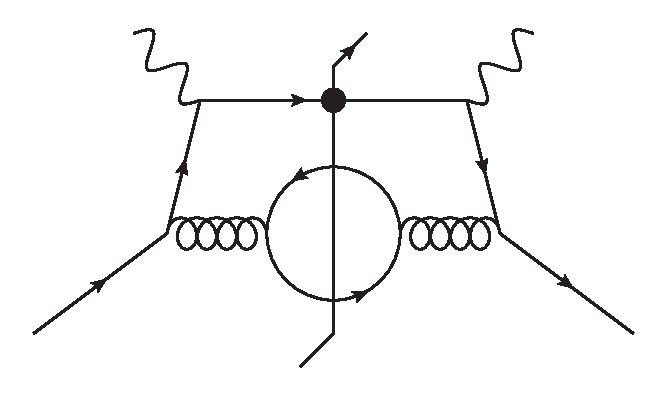
\includegraphics[scale=0.5]{chgA}
    \hspace{0.5cm}
    &
    \hspace{0.5cm}
    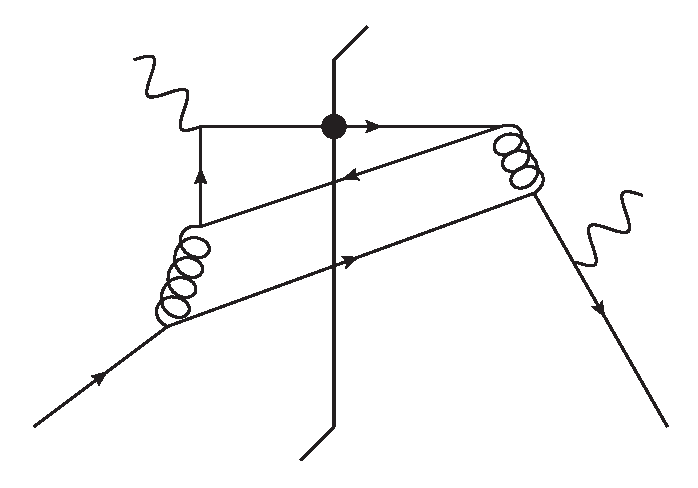
\includegraphics[scale=0.5]{chgB}
    &
    \hspace{0.5cm}
    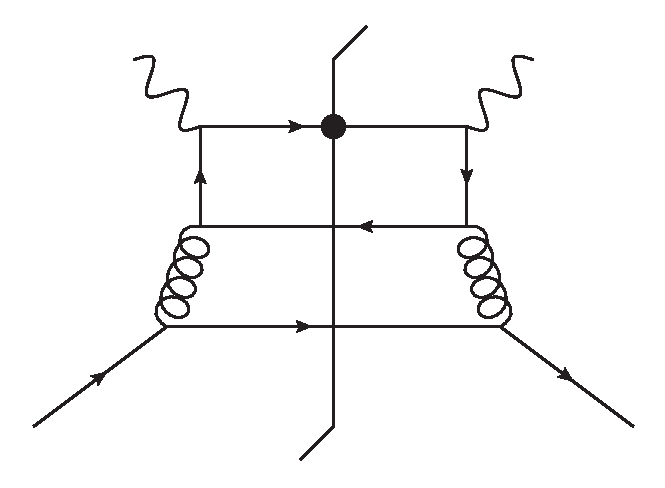
\includegraphics[scale=0.5]{chgC}
  \\
  (a) & (b) & (c)
  \end{tabular}
\caption{Examples of charge configurations $A$, $B$, and $C$. The solid black dot denotes the hadronizing parton.  
}
\label{chgconf}
\end{figure}
%---------------------

\begin{itemize}
\item \underline{Symbolic Calculation}:
\end{itemize}
The code for generating the cross section was obtained 
by directly evaluating the Feynman graphs involved at order $\alpha_s^2$, 
using utilities like qgraf, FORM, and Mathematica ({\color{red} citations}).
All of necessary codes and scripts are available ({\color{red} here}). 

The workflow showing their usage is shown in Fig.~\ref{workflow}
%---------------------
\begin{figure}[t]
\centering
    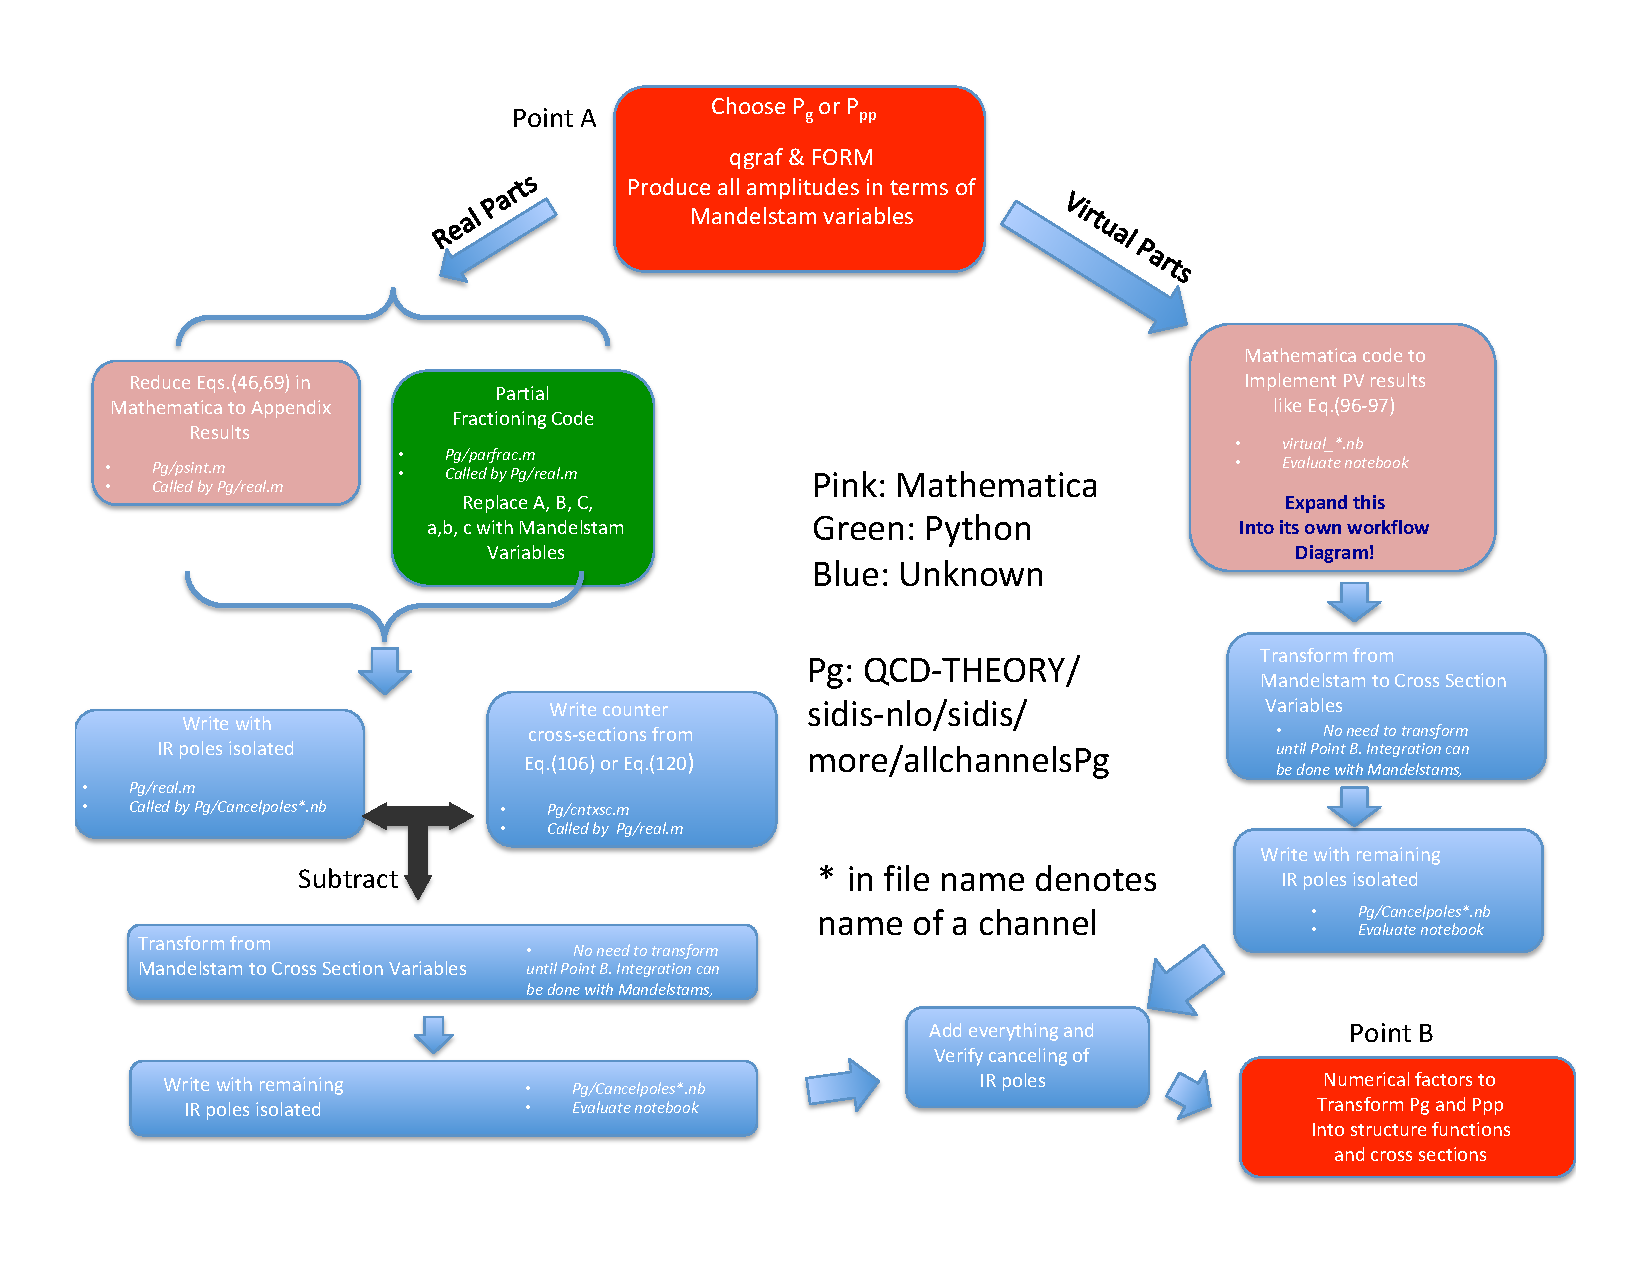
\includegraphics[scale=0.5]{workflow_master}
    \hspace{0.5cm}
\caption{Flow of tasks in the construction of cross section expressions.  
}
\label{workflow}
\end{figure}
%---------------------




\end{document}
